\documentclass{article}
\usepackage{graphicx}
\usepackage{float}
\usepackage{datetime}
\newdate{date}{30}{04}{2017}
\date{\displaydate{date}}

\begin{document}
\title{Study of TPLink router and Raspberry Pi on Prospect house power-line network}
\author{Abhinav Narain}
\maketitle
This report summarises results from experiments on TPLink router and
raspberry pi in 116 Prospect house.
\section{Experiment Design}
A device (TPLink router or Raspberry Pi) is plugged into live
power-socket next to EMI measurement equipment power-socket and
measurements are captured for different activities. Only few
activities are shown in the report for drawing conclusion.

\section{Results}
\subsection{TPLink}
\begin{figure}[H]
\centering
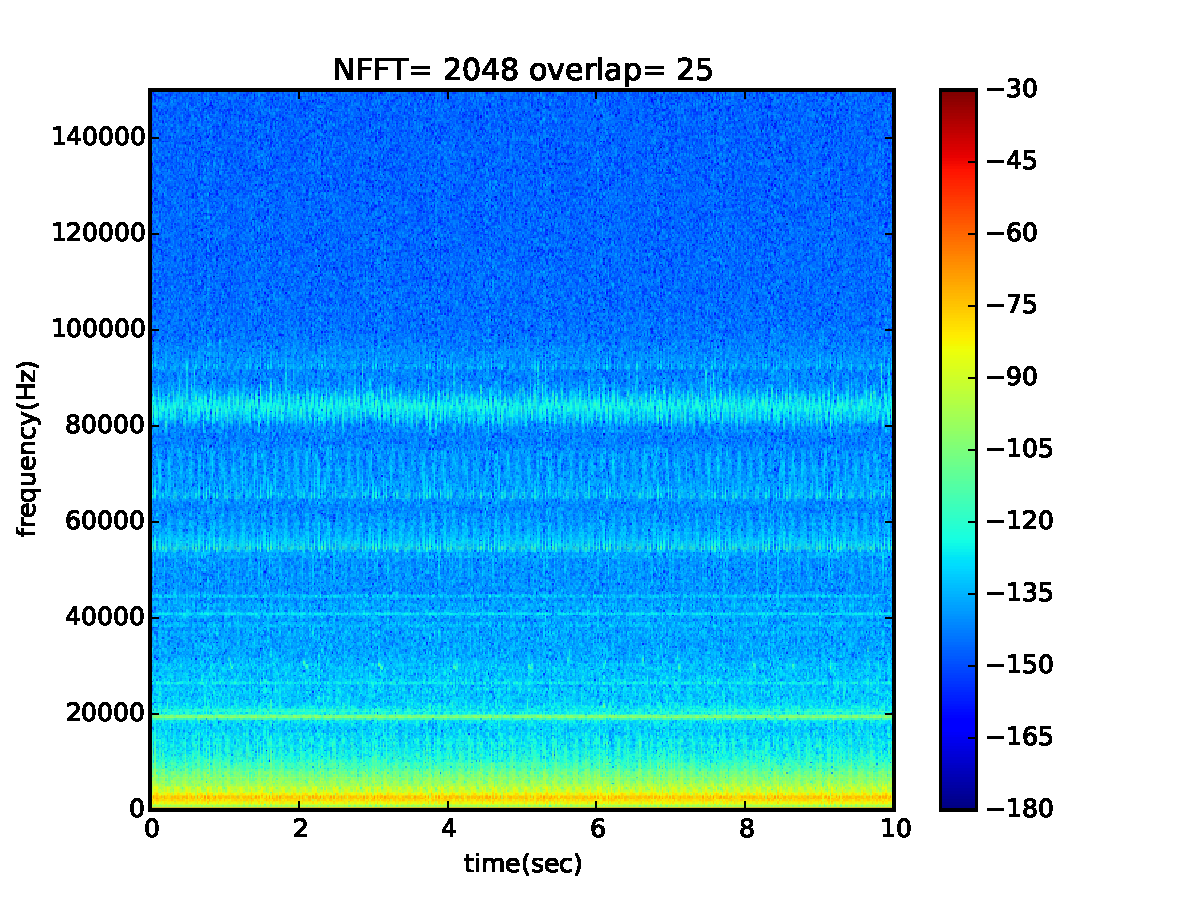
\includegraphics[width=\textwidth]{figures/lab/router_idle_2048.pdf}
\caption{Spectrogram of Idle (without any network/compute activity on the
  router) tplink router  in controlled environment}
\label{fig:t0}
\end{figure}

\begin{figure}[H]
\centering
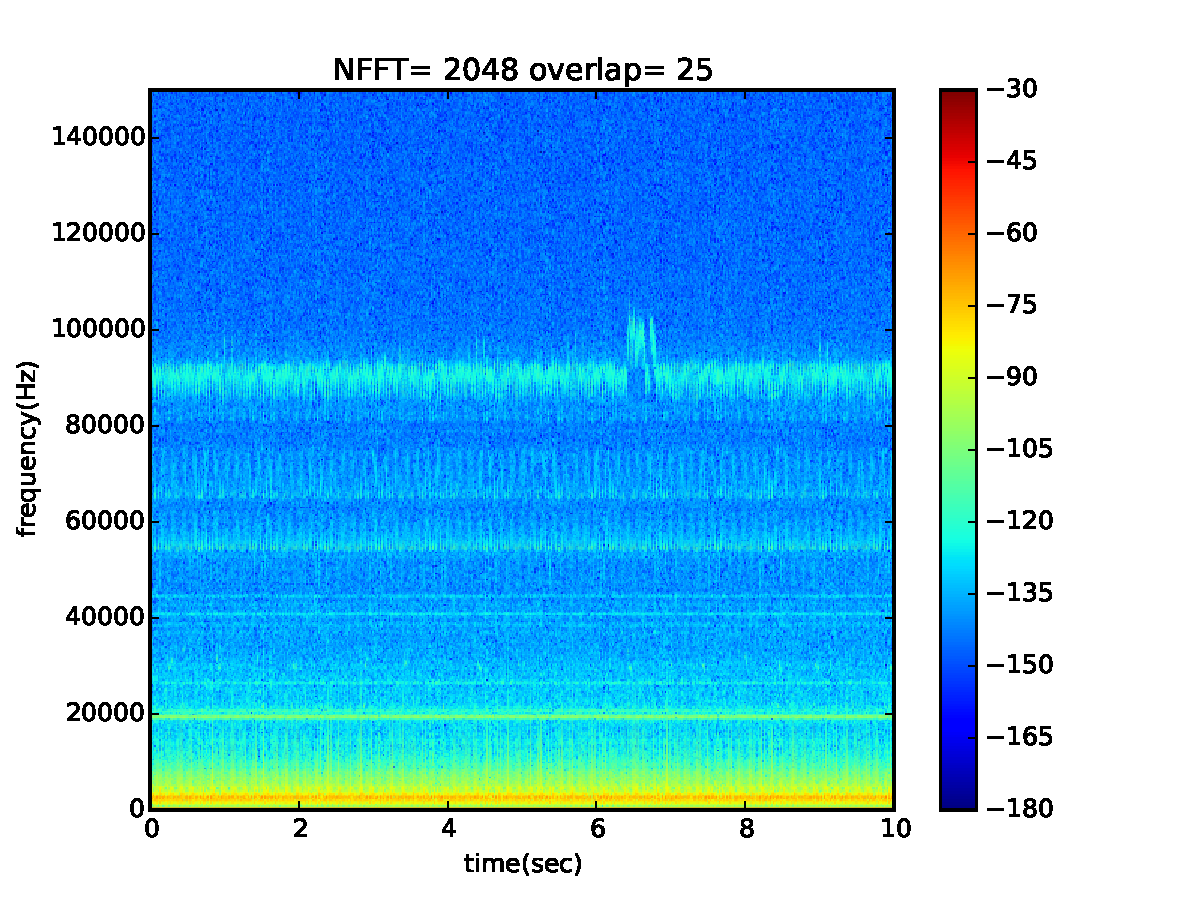
\includegraphics[width=\textwidth]{figures/lab/router_dns_2048.pdf}
\caption{Spectrogram of Mirai DoS (DNS) attack using tplink router in controlled environment}
\label{fig:tc1}
\end{figure}

\begin{enumerate}
\item Fig~\ref{fig:t0} and fig~\ref{fig:tc1} are spectrograms when
  experiments are conducted on separate power-line in controlled environment
\item  There is a marked difference in the change in frequency around
  80KHz to 90 KHz when a network intensive activity is started
\item The noise floor is low at the higher frequency range, compared
  to spectrogram~\ref{fig:t1} when measurements are conducted in house
  power-line network
\end{enumerate}

\begin{figure}[H]
\centering
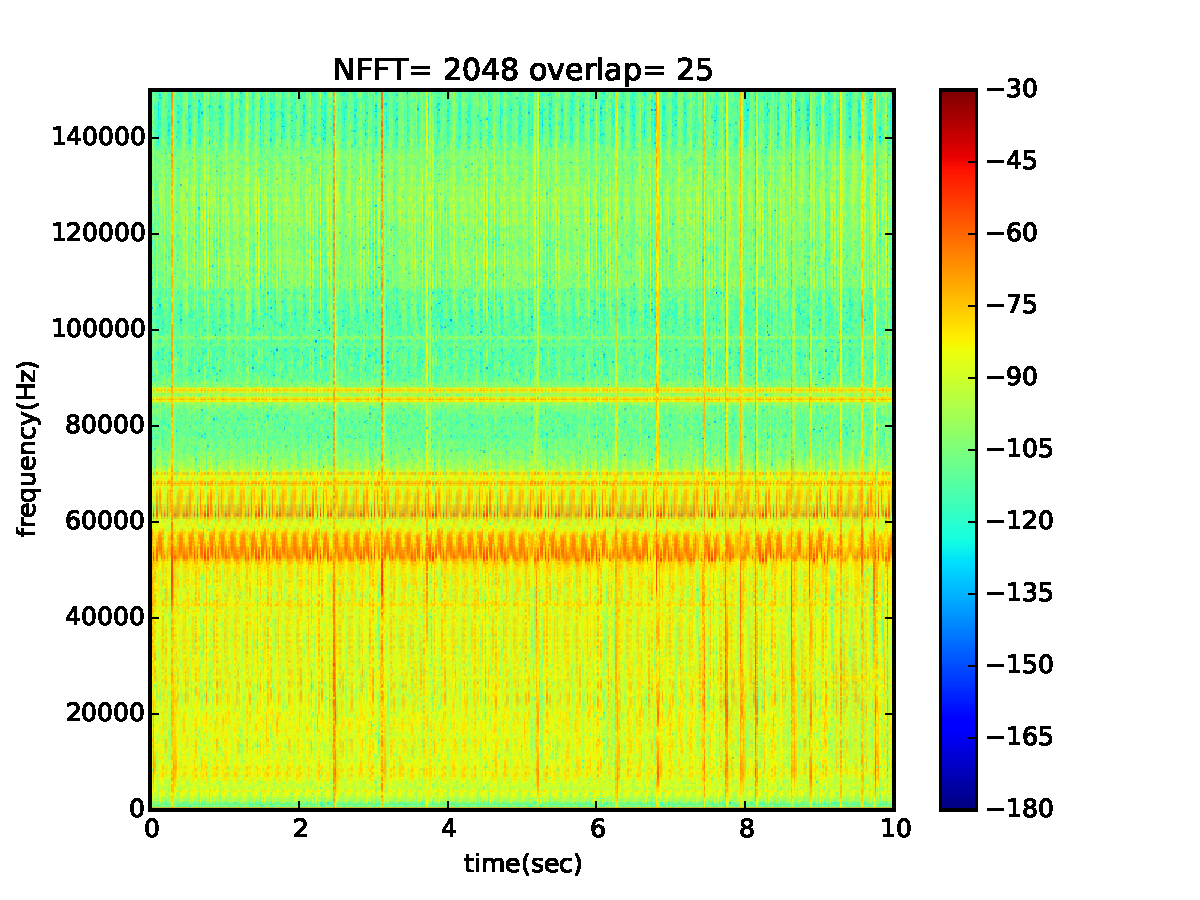
\includegraphics[width=\textwidth]{figures/prospect_tplink/prospect_tplink_idle_2048.pdf}
\caption{Spectrogram of Idle (without any network/compute activity
  started on the router) tplink router in Prospect house}
\label{fig:t1}
\end{figure}

\begin{figure}[H]
\centering
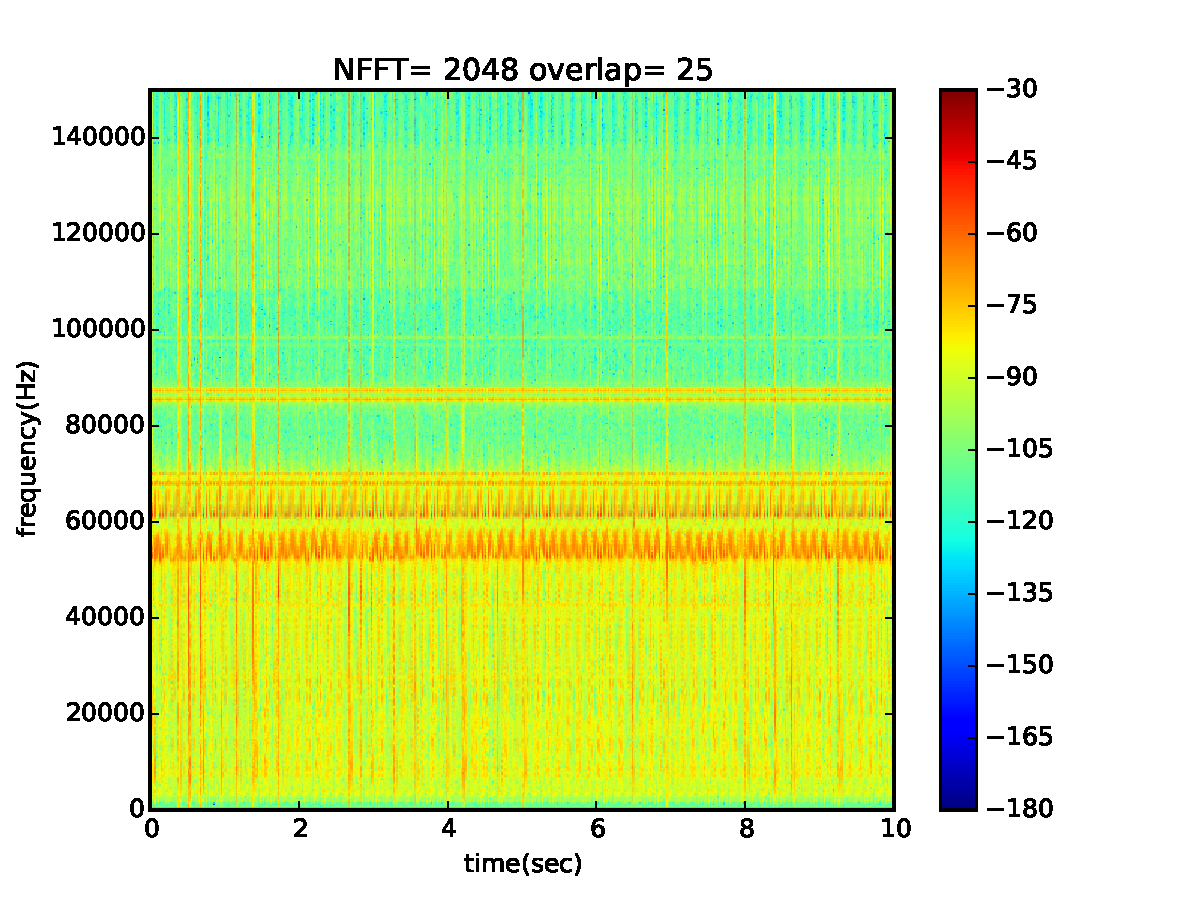
\includegraphics[width=\textwidth]{figures/prospect_tplink/prospect_tplink_mirai11_2048.pdf}
\caption{Spectrogram of Mirai DoS (DNS) attack using TPLink router in Prospect house}
\label{fig:t2}
\end{figure}

\begin{enumerate}
\item There is no change in EMI of the channel in Fig~\ref{t1} and
  Fig~\ref{t2}. Mostly because of the masking of the frequency range
  by other devices(unknown and already present) on the channel  
\item The overall noise on the channel is remarkably high, given the
  range of the scale is the same for all the spectrograms
\item Simple denoising technique of removing variance $\sigma\sqrt{\log{n}}$
(n is the number of samples) of the data was used, which as not
  yielded positive result in Fig~\ref{fig:t3}
\end{enumerate}

\begin{figure}[H]
\centering
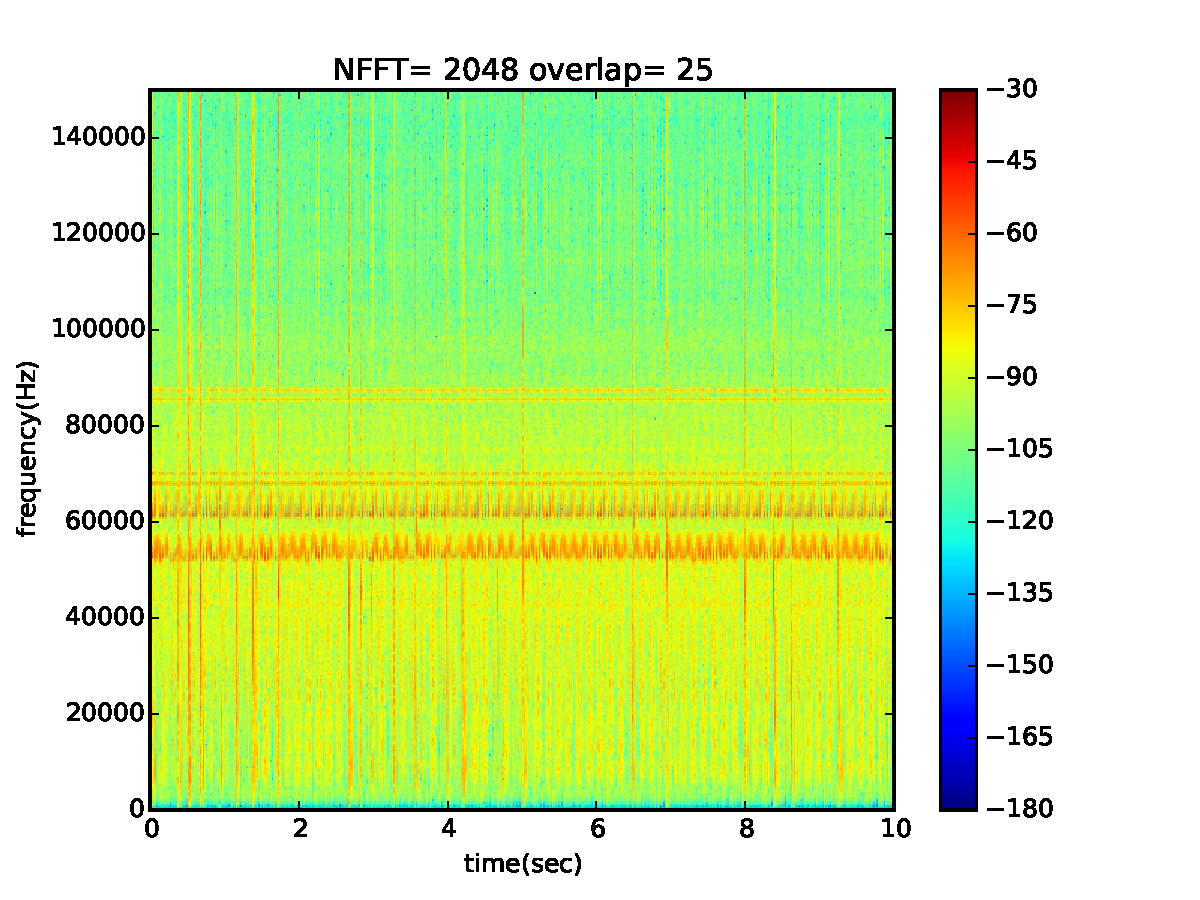
\includegraphics[width=\textwidth]{figures/prospect_tplink_den/prospect_tplink_mirai11_den_2048.pdf}
\caption{Spectrogram of denoising Mirai DoS (DNS) activity using TPLink router in Prospect house}
\label{fig:t3}
\end{figure}

\subsection{Raspberry Pi}
\begin{figure}[H]
\centering
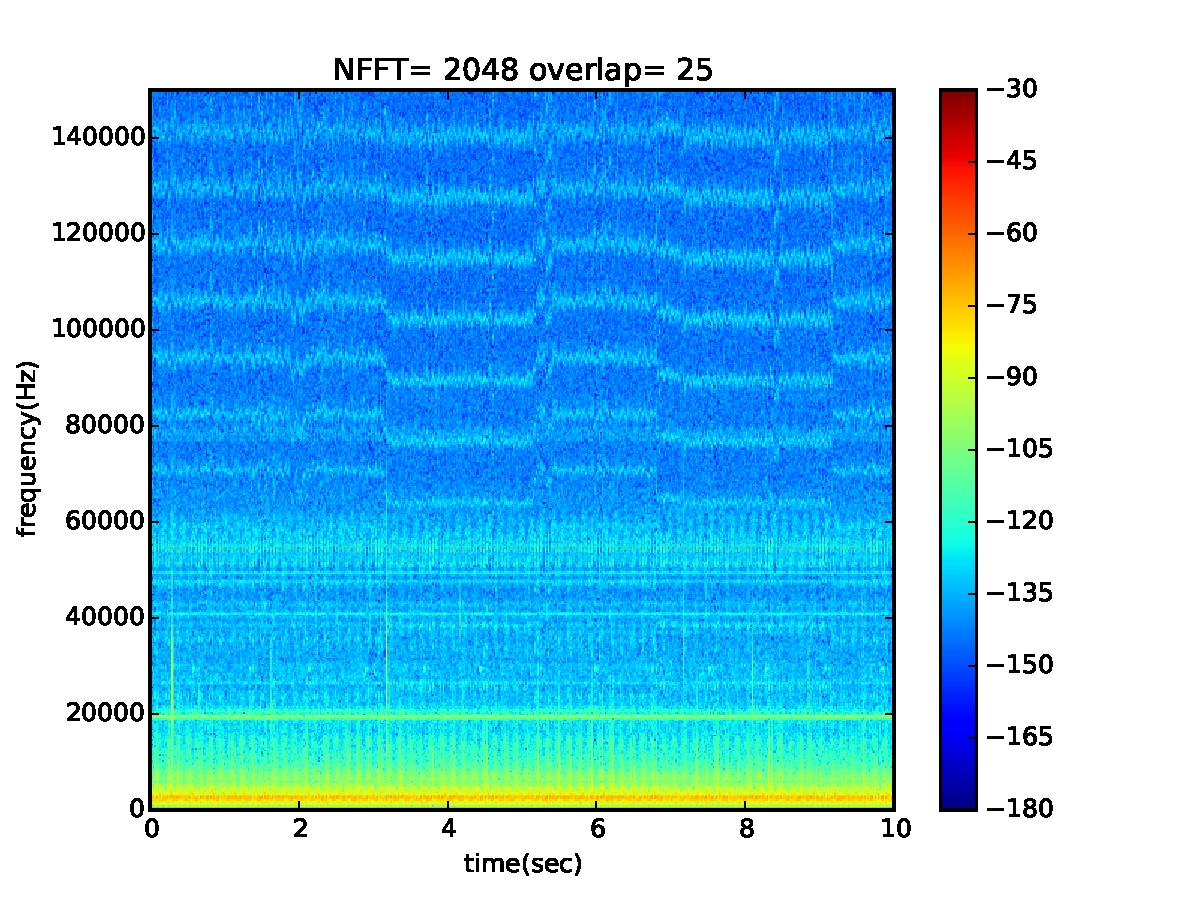
\includegraphics[width=\textwidth]{figures/lab/raspi_litecoin_2048.pdf}
\caption{Spectrogram of raspberry Pi running Litecoin miner in controlled environment}
\label{fig:t4}
\end{figure}

\begin{figure}[H]
\centering
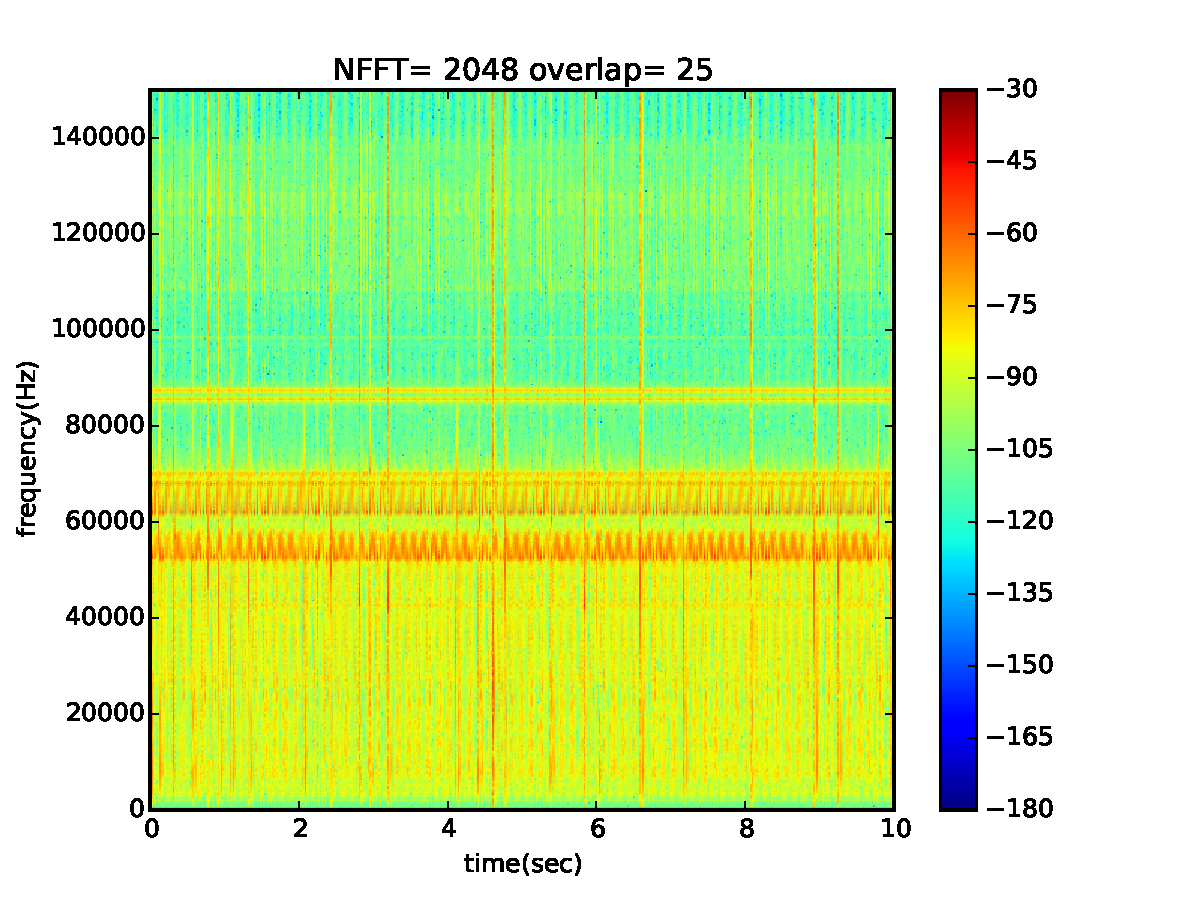
\includegraphics[width=\textwidth]{figures/prospect_raspi/prospect_raspi_miner_2048.pdf}
\caption{Spectrogram of mining activity on raspberry Pi. There is no
  noticeable difference as the expected frequencies around 80 KHz are masked.}
\label{fig:t5}
\end{figure}

\begin{figure}[H]
\centering
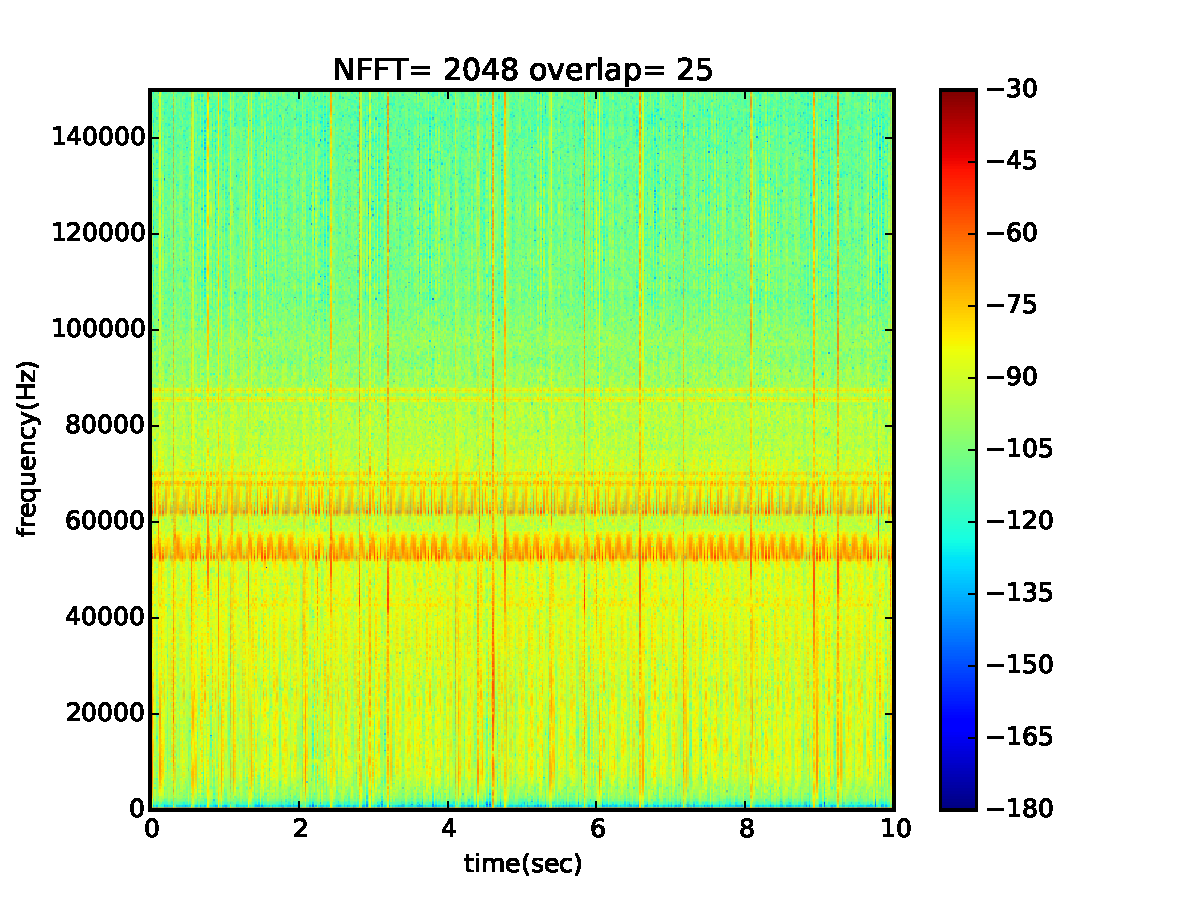
\includegraphics[width=\textwidth]{figures/prospect_raspi_den/prospect_raspi_miner_den_2048.pdf}
\caption{ Spectrogram of denoising Litecoin miner activity on
  raspberry Pi}
\label{fig:t6}
\end{figure}

\begin{enumerate}
\item There is no change in EMI of the channel in Fig~\ref{t5} as
  expected in  Fig~\ref{t4}. This is due to masking of the frequency range
  by other devices on the channel  
\item The overall noise on the channel is remarkably high, given the
  range of the scale is the same for all the spectrograms
\item Simple denoising technique of removing variance $\sigma\sqrt{\log{n}}$
(n is the number of samples) of the data was used, which as not
  yielded positive result in Fig~\ref{fig:t6}
\end{enumerate}

\end{document}
